%%%%%%%%%%%%%%%%%%%%%%%%%%%%%%%%%%%%%%%%%%%%%%%%%%%%%%%%%%%%%%%%%%% 
%                                                                 %
%                            CHAPTER THREE                        %
%                                                                 %
%%%%%%%%%%%%%%%%%%%%%%%%%%%%%%%%%%%%%%%%%%%%%%%%%%%%%%%%%%%%%%%%%%% 
 
\chapter{Infrared Spectroscopy of Clay Minerals}

\begin{figure}
	\centering
	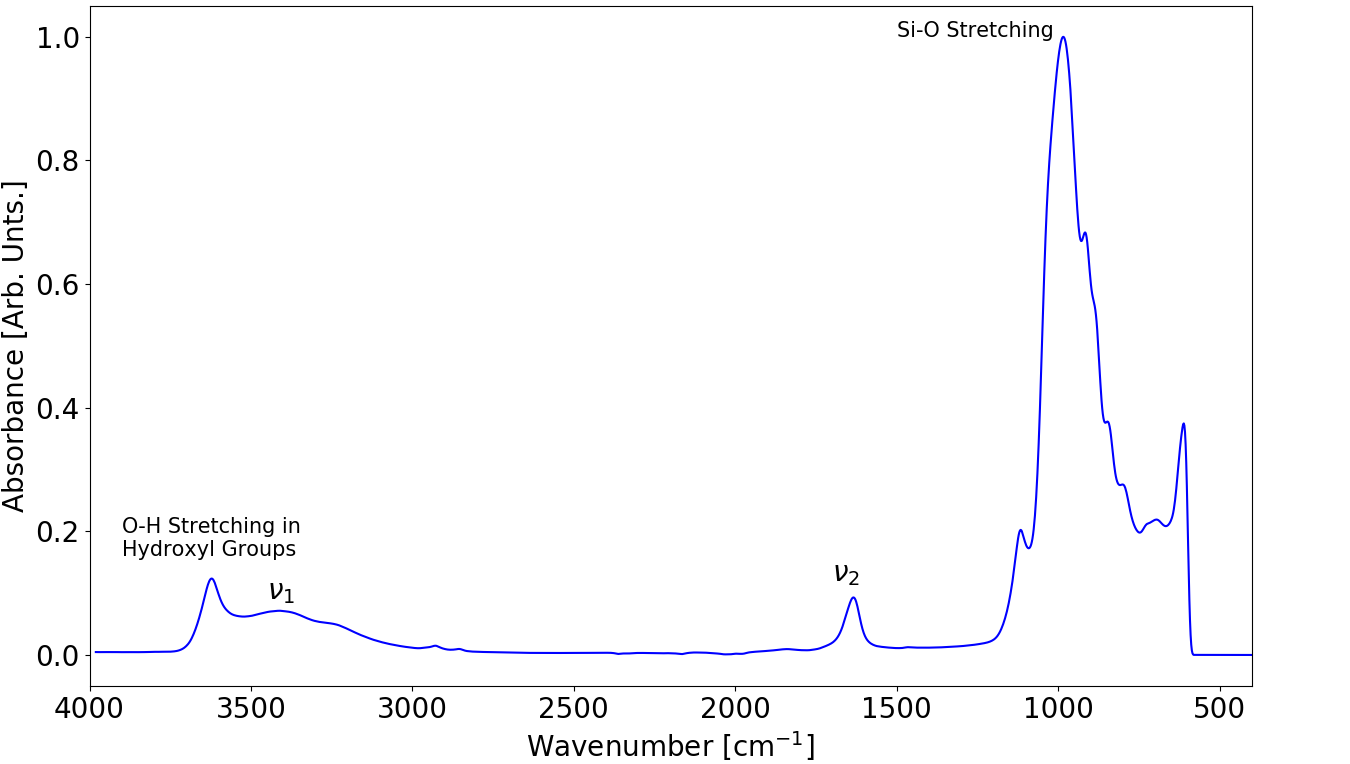
\includegraphics[scale=0.5]{images/spectrum_labels.png}
	\caption{Complete IR spectrum of a Li$^{\bm{+}}$ montmorillonite sample prepared at a pH of 7.}
	\label{fig:spectrum}
\end{figure}

\section{Infrared Spectrum of Montmorillonite}
An example of a typical infrared spectrum of a montmorillonite sample is provided in Figure~\ref{fig:spectrum}. In general, there are three regions of interest in the $500cm^{-1}$ - $4000cm^{-1}$ band. The first such region occurs between $500cm^{-1}$ and $1300cm^{-1}$. There are many overlapping absorbance bands within this region, all of which are attributed to vibrational modes of the clay structure itself. Within the scope of this work, these modes are of little interest, as we are focused primarily on the effects on water. It is also difficult to measure effects on these modes as their exact characteristics are heavily dependent on the composition, and therefore the source, of the clay samples \cite{madejova2001baseline}. One overarching trait of importance to this work however is the largest absorbance maximum in this region (and in the provided spectrum as a whole). This absorbance band is attributed to the Si-O stretching mode of the silica molecules in the clay \cite{madejova2001baseline}. This maximum is always the majorant over the spectrum, and is used in this paper to normalize our collected spectra, so that comparisons may be made between them. Apart from this, no analysis has been conducted on the absorbance bands located in this region.

Second, is the region between $1500cm^{-1}$ and $1800cm^{-1}$ containing one absorbance maximum, usually located at $1633cm^{-1}$. As previously mentioned, this is attributed to the bending mode of the intercalated water ($\nu_2$) \cite{madejova2003ftir}, \cite{madejova2001baseline}, \cite{bishop1994infrared}, \cite{johnston1992vibrational}, \cite{xu2000infrared}. This is one of the three bands which will be of interest for the remainder of this work.

\begin{figure}
	\centering
	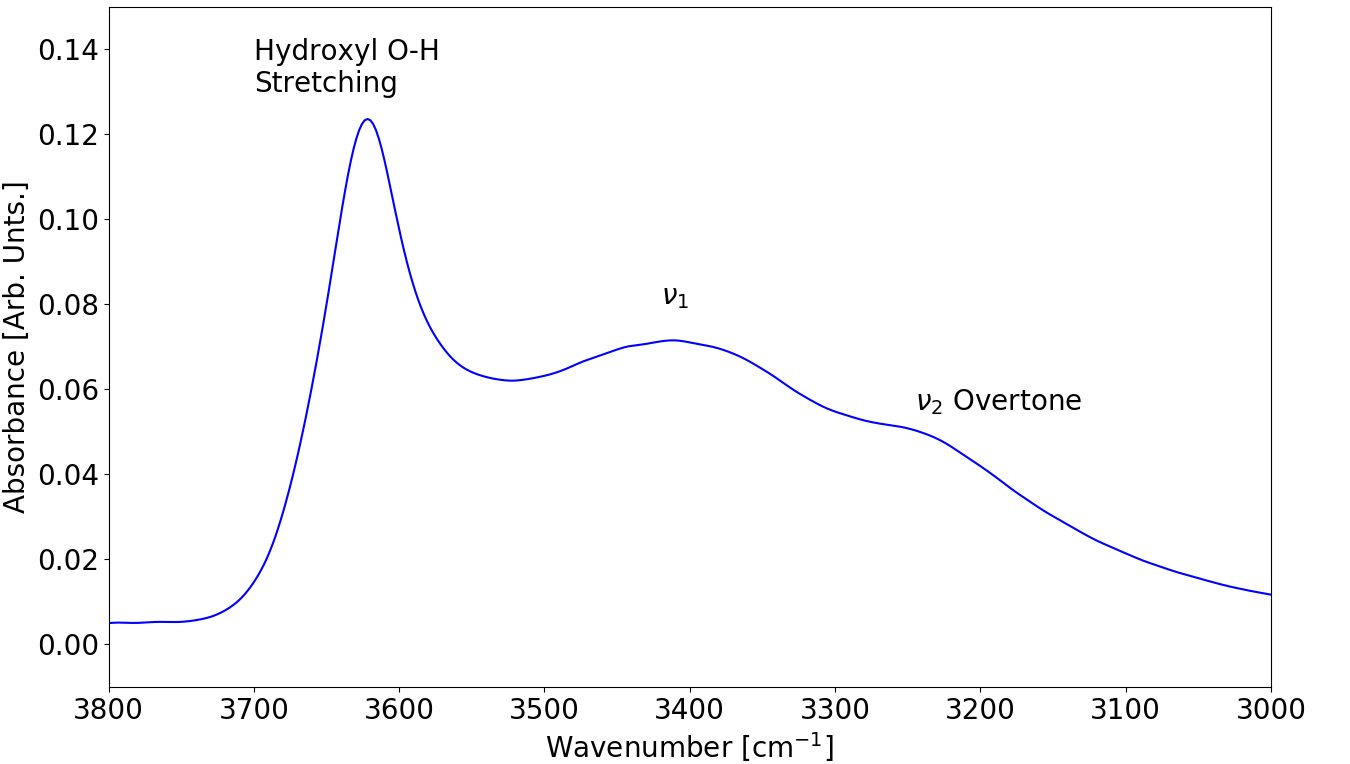
\includegraphics[scale=0.5]{images/water_peaks.png}
	\caption{3800cm$^{-1}$ - 3000cm$^{-1}$ region of montmorillonite infrared spectrum.}
	\label{fig:water_peaks}
\end{figure}

The third region of interest is between $3000cm^{-1}$ and $3800cm^{-1}$. In this band, there are three overlapping absorbance maxima. The most prominent and well defined is located at approximately $3620cm^{-1}$, and is attributed to the O-H stretching mode of the hydroxyl groups which are part of the clay lattice itself. The second which is much broader and located around $3410cm^{-1}$ is due to the symmetric stretching mode ($\nu_1$) of the O-H bond in the water molecules \cite{madejova2001baseline}. To the right, at $3242cm^{-1}$ is an overtone of the $\nu_2$ mode previously described \cite{xu2000infrared}. Of these three absorbance bands, the two which are pertinent to this work are the O-H stretching mode of the hydroxyl groups, and the $\nu_1$ mode of the intercalated water. Although the absorbance peak generated by the principal tone of the $\nu_2$ mode is tracked throughout the course of this experiment, the overtone was not considered in the analysis. This is due to the difficulty in fitting this small and less prominent absorbance peak, and because it is assumed that any variations in the $\nu_2$ mode of the water would present themselves in the resonance located at $1633cm^{-1}$.

Previously, it was briefly mentioned that all spectra collected in this work were normalized to the majorant absorbance peak of the Si-O stretching mode. While the structure and composition of montmorillonites varies (even within samples taken from the same location), it has been shown previously by Wilke, Aldersley, and Joshi that that the average compositions are similar enough that an appropriate choice for normalization would be the Si-O absorbance maximum \cite{wilke2016}. It is also easy to find and has a very consistent frequency between samples, making this an ideal choice as well. Normalizing the spectra is important, as the height of the absorbance maxima corresponding to $\nu_1$ and $\nu_2$ give an indication as to the quantity of water present, relative to other samples. The more water present in a sample, the higher the absorbance for the bands corresponding to modes occurring in the intercalated water. Therefore, as the level of hydration decreases, the heights of the $\nu_1$, $\nu_2$, and $\nu_2$ overtone absorbance bands also decrease \cite{madejova2003ftir}, \cite{bishop1994infrared}, \cite{johnston1992vibrational}, \cite{xu2000infrared}. While the height of these maxima and the hydration level of the clay are not specifically considered in this experiment, the effects of the hydration level on the frequencies of these vibration modes will be discussed in the upcoming section, and the ability to make general comparisons between spectra is of value.


\section{Previous Investigations}
\subsection{Effects of Hydration Level}
There have been many previous studies which examine the effects of hydration level on the stretching and bending modes of the intercalated water. Johnston, Sposito, and Erickson studied the effects of hydration on the water deformation mode ($\nu_2$) in their 1992 paper. In that work, it was found that regardless of which exchangeable cation was present in the clay sample, moving from a hydration level of 0 to approximately 10-15 H$_2$O molecules per cation, the frequency of the $\nu_2$ mode also increases. For a hydration of 15 or more H$_2$O molecules per cation, the frequency change begins to level off, and is similar to that of bulk water \cite{johnston1992vibrational}.

Bishop, Pieters, and Edwards in 1994 conducted a similar work, but expanded analysis to all bands attributed to water in the infrared and near infrared regions as well. Their results supported those of Johnston, Sposito, and Erickson, indicating that for Na montmorillonite, an observed shift in the $\nu_2$ band from $1617cm^{-1}$ to $1630cm^{-1}$ occurred as the sample was hydrated. Contrasting the behavior of the $\nu_2$ band, the absorbance maximum due to the $\nu_1$ band decreases with frequency as the hydration increases. No correlation was found between the band attributed to O-H stretching of structural hydroxyl groups and the hydration level \cite{bishop1994infrared}.

These two previous papers are further backed by a third, from 2000 written by Xu, Johnston, Parker, and Agnew. The results of Johnston's initial 1992 paper further support this work, and again show a trend of increasing frequency for the $\nu_2$ band from approximately $1625cm^{-1}$ to $1636cm^{-1}$ for Na and Li montmorillonites. At levels of hydration $>$ 10 water molecules per cation, the frequency again appears to remain constant. This paper also provided a more in depth analysis of the $\nu_1$ absorbance band as a function of water content as well. For all cations tested, the frequency of the symmetric stretching mode decreased with increasing water content. Na and Li samples tended to shift from around $3430cm^{-1}$ to $3420$ or $3415cm^{-1}$ when being hydrated from $<$ 5 water molecule per cation, to 15 molecules per cation. While this work did not specifically analyze the structural O-H stretching mode at $3620cm^{-1}$, based on their provided graphs, it would appear that little variation was present in this mode \cite{xu2000infrared}.

While specific values may vary slightly between these works, the general observations are consistent throughout. In general it is clear that more intercalated water causes an increase in the frequency of the $\nu_2$ mode, and a decrease in the frequency of the $\nu_1$ mode. Both the papers by Johnston and Xu propose the explanation that a decrease in the frequency of the $\nu_2$ mode under dehydration indicates that there are fewer hydrogen bonds forming between water molecules, and that the remaining molecules are then clustered around the exchangeable cations \cite{xu2000infrared}, \cite{johnston1992vibrational}. The paper by Johnston goes further in its explanation, stating that the water molecules conglomerated around the cation become polarized, and that this should be accompanied by an increase in the frequencies of the $\nu_1$ and $\nu_3$ modes \cite{johnston1992vibrational}. Though they were not able to make such observations at the time, the papers by Bishop and Xu both observe these traits in combination, supporting the provided explanation.

\subsection{Effects of Interlaminar Cation}
As previously explained, the amount of intercalated water has an effect on the frequencies of the symmetric stretching and deformation modes of this water. The interlaminar cation which is present also has an effect on these frequencies, due to both its size and valence. Furthermore, some of the previously discussed hydration properties may also be affected by the species of exchangeable cation present in the sample. Such effects shall briefly be discussed here.

In Johnston, Sposito, and Erickson's previously mentioned paper, the frequency range of the $\nu_2$ mode was examined at varying hydration levels for samples with Na, K, Co, and Cu cations. From their presented data it can be seen that upon reaching the hydration level at which the $\nu_2$ mode no longer changed with hydration, Co and Cu samples both had frequencies at approximately 1633$cm^{-1}$ to 1635$cm^{-1}$. These are slightly lower than the values for K and Na samples which were at 1637$cm^{-1}$ and 1640$cm^{-1}$ respectively \cite{johnston1992vibrational}. Bishop, Pieters, and Edwards observed that higher energies were observed for the water deformation mode for exchangeable cations which has a higher polarizing ability (i.e. higher charge and smaller radius). Similarly, it was postulated that as the polarizing ability of the cation is increased, the energy of the $\nu_1$ mode should decrease. This was supported in their observations for samples which had a higher water content, but for lower hydration levels, this appeared to not hold true \cite{bishop1994infrared}. Xu, Johnston, Parker, and Agnew also observed a strong dependence of the $\nu_2$ mode on the valence of the exchangeable cation. Na and Li samples reached a stable frequency at 1636$cm^{-1}$, while Mg and Ca samples were at slightly lower energies, of 1633$cm^{-1}$. For the $\nu_1$ mode, Na and Li samples had frequencies of approximately 3420$cm^{-1}$ at hydration of $>$ 10 $H_2O$ molecules per cation, while Ca and Mg samples were slightly lower, at 3415$cm^{-1}$ and 4505$cm^{-1}$ respectively \cite{xu2000infrared}.

With these direct effects due to the interlaminar cation described, one must also remember that the species of cation has an effect on the hydration level of the clay. As Jacques Méring described in his 1964 paper, montmorillonites which contain K as the exchangeable cation will usually only develop a monolayer of water between clay sheets. This is a general property as one moves down the periodic table, using cations with a larger radius, as compared to atoms such as Na and Li \cite{mering1964gonflement}. This difficulty in hydration means that the cation which is present could also lead to secondary effects which occur due to the hydration level, as discussed in the previous section.

\section{Effects of the Variation of pH}
To better understand the role the pH of a montmorillonite sample plays in this system, the following experiment was devised to better understand how the pH affects the symmetric stretching, and deformation modes of the water, and also of the O-H stretching mode in the structural hydroxide groups. To do this, series of samples were produced, with one series corresponding to one clay mine, and one exchangeable cation (Li, Na, or K). Within a series, 15 sample disks were produced, each corresponding to a different pH value between 3 and 10, using a 0.5 interval. Infrared spectra of each sample were then collected and analyzed. What remains of this chapter is devoted to an explanation of the methodology used, and the presentation of the results.

\subsection{Experimental Methods}
\subsubsection{Clay Sample Preparation}
The samples used through the course of this experiment were produced using montmroillonite acquired from the American Colloid Company, originating from the Belle Fourche A, C, and F clay mine beds, in addition to samples from the Miniota and Treherne mine beds. Homoionic samples with Li, Na, and K as the exchangeable cation were prepared by mixing the clays with chloride salts associated with the desired cation. All of the sample disks in a series were produced from the resulting clay, which was then titrated to the desired pH, using the methodology described by Banin et. al. \cite{banin1985ph}. After a sample at each desired pH level for a sample series was produced, the clay was centrifuged, then freeze dried, as prescribed by Aldersley, Joshi, Price, and Ferris \cite{aldersley2011role}.

With each series of clay powders produced, a clay pellet was produced for each pH in each sample series produced. The methodology used to produce these pellets is identical to that previously described in chapter 2. As before, no KBr was mixed with the clay powder. After each pellet was formed, it was placed in its own vial, and left in the lab at room temperature and room humidity ($p/p_0\approx 0.4 - 0.6$).

\subsubsection{Collection of Infrared Spectra}
For each sample prepared, two infrared spectra were taken using a Nicolet 4700 ATR-FTIR device. A resolution of 2$cm^{-1}$ was used for all measurements, and spectra were taken over the interval of $4000cm^{-1}$ - $500cm^{-1}$. To collect an infrared spectrum of a sample, the sample stage was first cleaned using isopropyl alcohol and disposable lab wipes. The desired clay pellet was then removed from its vial, and placed on the platform, and centered over the crystal. A press was then manually lowered onto the pellet, maintaining contact between the clay pellet and the crystal of the spectrometer. While the pellets are in general rather sturdy, the pressure required over the small surface area would sometimes cause the pellets to break in half, crumble, or crack. With a bit of finesse and practice, the maximum amount of pressure possible without breaking the clay pellet was applied. One may closely observe the surface of the pellet and see deformations and cracks begin to form, so it is known when to stop applying pressure. Despite the care used in this process, samples inevitably cracked, and crumbled. When this occurred, the press was removed, and the largest remaining piece of the sample was then placed over the crystal, and the press was again gently re-applied.

After one spectrum was completed, the press would be removed, and the sample (or its remains) would be reoriented to obtain a second spectrum in a different location on the pellet. After this, the sample and its remains would be collected and replaced in the vial. The stage and press would be washed again with isopropyl alcohol between each sample. Occasionally, a spectrum would be collected which did not resemble a standard infrared spectrum of montmorillonite. It was found that this was due to a lack of sufficient contact between the sample, and the spectrometer crystal on the stage. In this case, the sample was re-positioned, and more pressure was applied using the press.

\subsection{Results}

\subsubsection{Data Analysis}
\begin{figure}
	\centering
	\begin{subfigure}{1\textwidth}
		\centering
		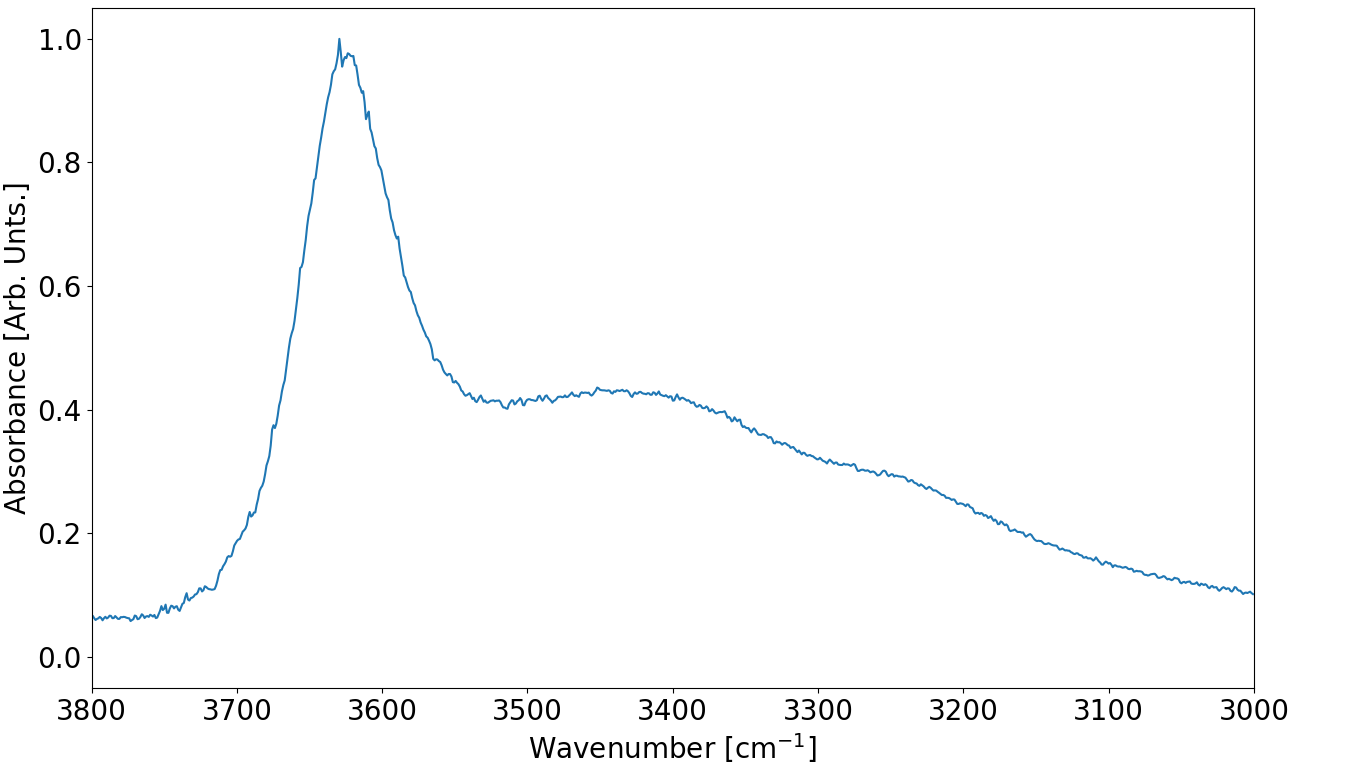
\includegraphics[scale=0.5]{images/raw_spectrum_noise.png}
		\caption{Raw sample spectrum with high frequency noise.}
		\label{fig:spectrum_noise}
	\end{subfigure}\newline
	\begin{subfigure}{1\textwidth}
		\centering
		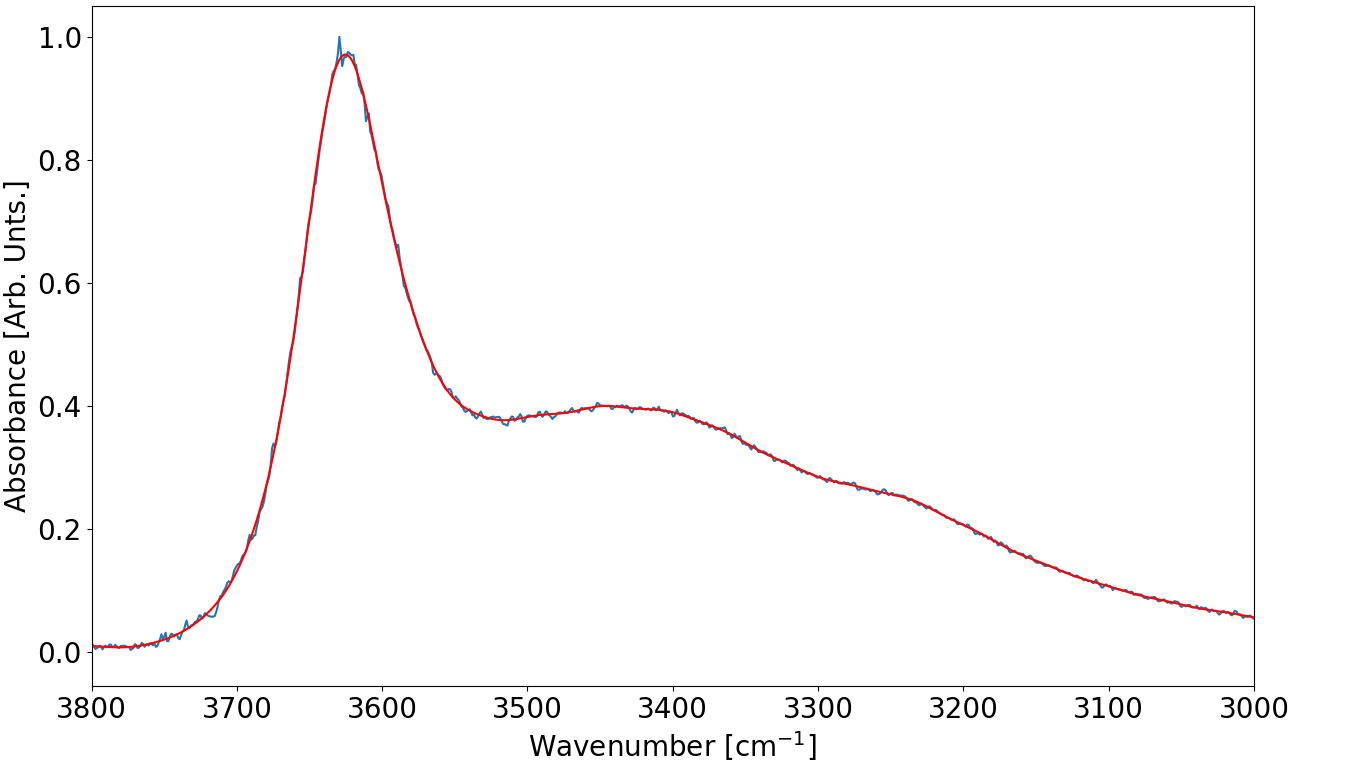
\includegraphics[scale=0.5]{images/filtered_peaks.png}
		\caption{Fourier filtered spectrum plotted over original spectrum from above.}
		\label{fig:filtered_specctrum}
	\end{subfigure}
	\caption{Raw and filtered spectrum of a pH 9.5 Na exchanged sample from 3800cm$^{-1}$ to 3000cm$^{-1}$.}
	\label{fig:raw_spectrum}
\end{figure}

Upon completion of scanning all samples twice, there were approximately 390 spectra which had to be analyzed. A resulting raw spectrum may be viewed in Figure~\ref{fig:spectrum_noise}. While this spectrum clearly has the overall characteristics of a montmorillonite infrared spectrum between 3000$cm^{-1}$ and 3800$cm^{-1}$, as initially presented by Figure~\ref{fig:water_peaks}, a high frequency noise is present in the spectrum. This noise made it difficult to pinpoint the frequencies of the $\nu_1$ and structural O-H stretching modes. Initially, a simple local averaging algorithm was used to smooth the data, but this lead to a slight loss of structure to the overall shape of the spectrum, especially in the region below 1000$cm^{-1}$, due to the number of small absorbance maxima in those areas. In an effort to preserve overall form, while also removing the high frequency noise, effectively smoothing the data, a Fourier filter was applied to the spectra. To accomplish this, the two regions of interest were each treated separately in the following manner: a linear background was subtracted from the region, using the end points of those regions. A Fourier filter was then applied, using a cutoff frequency of 0.024$cm$. This value was determined by trial and error, looking at the resulting form of the spectrum and adjusting the frequency until a spectrum which looked sufficiently smooth, while also conserving the overall form was found. Appendix~\ref{appendix:fft_filter} has the python script containing the Fourier Filter algorithm used. A filtered spectrum plotted over the original is provided in Figure~\ref{fig:filtered_specctrum}. As these filtered spectra were easier to find absorbance maxima locations from, they were used to conduct all the analysis, and find all frequencies.

Once filtered, the frequencies of the three local absorbance maxima of interest were obtained by fitting a Gaussian curve to the location of the maximum. Due to the large number of spectra collected and the time this would take to obtain all the data conducting the analysis by hand in software such as OriginPro, a script was written in Python to automate this process.

\subsubsection{Variations Due to pH}
\begin{figure}
	\centering
	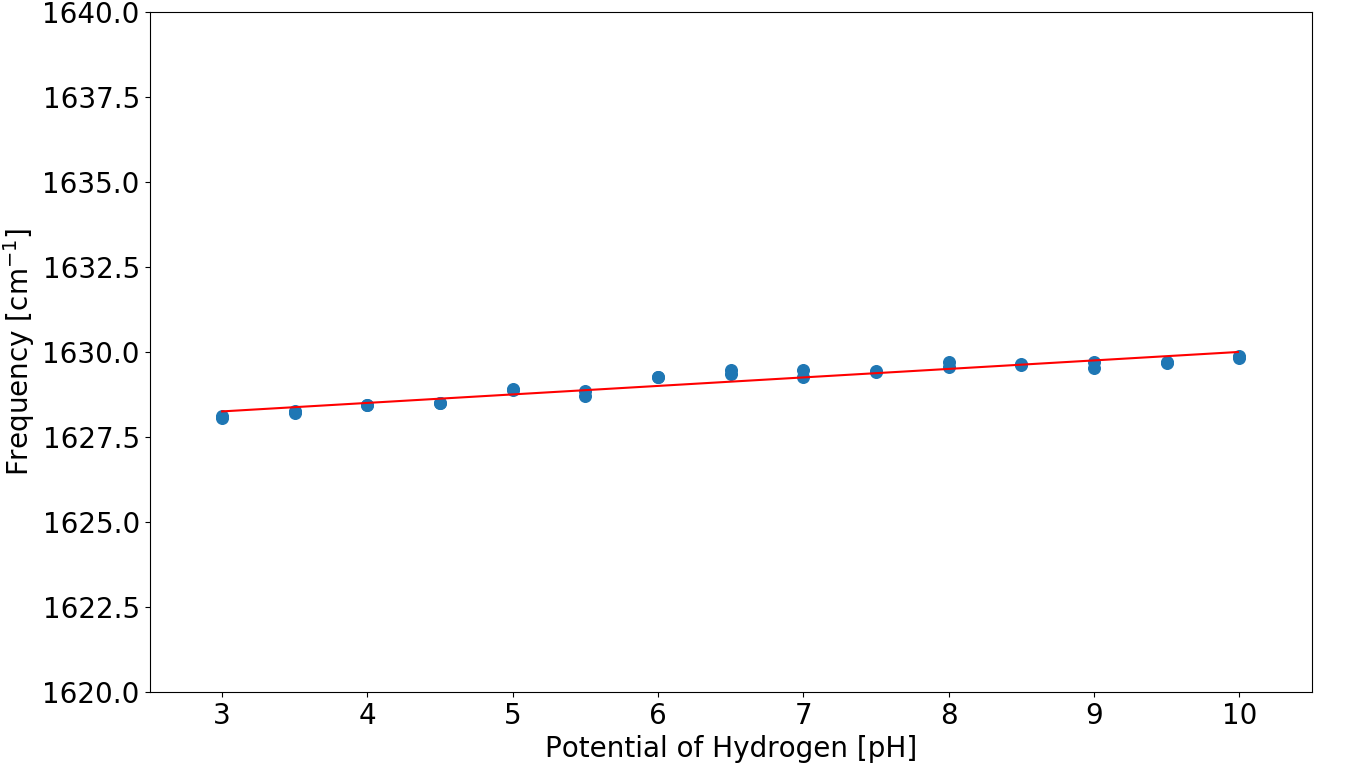
\includegraphics[scale=0.5]{images/deformation_shift.png}
	\caption{Water deformation mode of the Li sample series from Belle Fourche bed F as a function of the pH. Each 0.5 pH interval has two data points. Linear regression provided only as a guide to the eye.}
	\label{fig:deformation_shift}
\end{figure}
Once all the water vibration frequencies were determined for all samples in a series, the frequency of each of the three modes of interest was plotted against the pH of the sample. Looking at Figure~\ref{fig:deformation_shift}, one may see such a plot for the $\nu_2$ water deformation mode. From pH 3 to pH 10, there is an average shift in frequency of just under 2$cm^{-1}$. This observation was consistent between not only all Li sample series, but also for all series from the other two cations. One is directed to Table~\ref{tab:deformation_shifts} to see at what frequencies this shift occurred for each sample series.
\begin{table}
	\centering
	\caption{The frequencies over which the shift in the $\nu_2$ mode occurs when moving from pH of 3 to 10 for all sample series.}
	\label{tab:deformation_shifts}
	\begin{tabular}{|c||c|}
		\hline
		\textbf{Sample Series} & \textbf{Frequency Range of $\bm{\nu_2}$ Mode [$\bm{cm^{-1}}$]} \\
		\hline
		\hline
		Li $_A$ & 1628 - 1630 \\
		\hline
		Li $_C$ & 1628 - 1630 \\
		\hline
		Li $_F$ & 1628 - 1630 \\
		\hline
		Li $_T$ & 1628 - 1630 \\
		\hline
		Na $_A$ & 1628 - 1630 \\
		\hline
		Na $_C$ & 1628 - 1630 \\
		\hline
		Na $_F$ & 1628 - 1630 \\
		\hline
		Na $_M$ & 1628 - 1630 \\
		\hline
		Na $_T$ & 1628 - 1630 \\
		\hline
		K $_A$ & 1628 - 1630 \\
		\hline
		K $_C$ & 1628 - 1630 \\
		\hline
		K $_M$ & 1628 - 1630 \\
		\hline
		K $_T$ & 1628 - 1630 \\
		\hline
	\end{tabular}
\end{table}

\begin{figure}
	\centering
	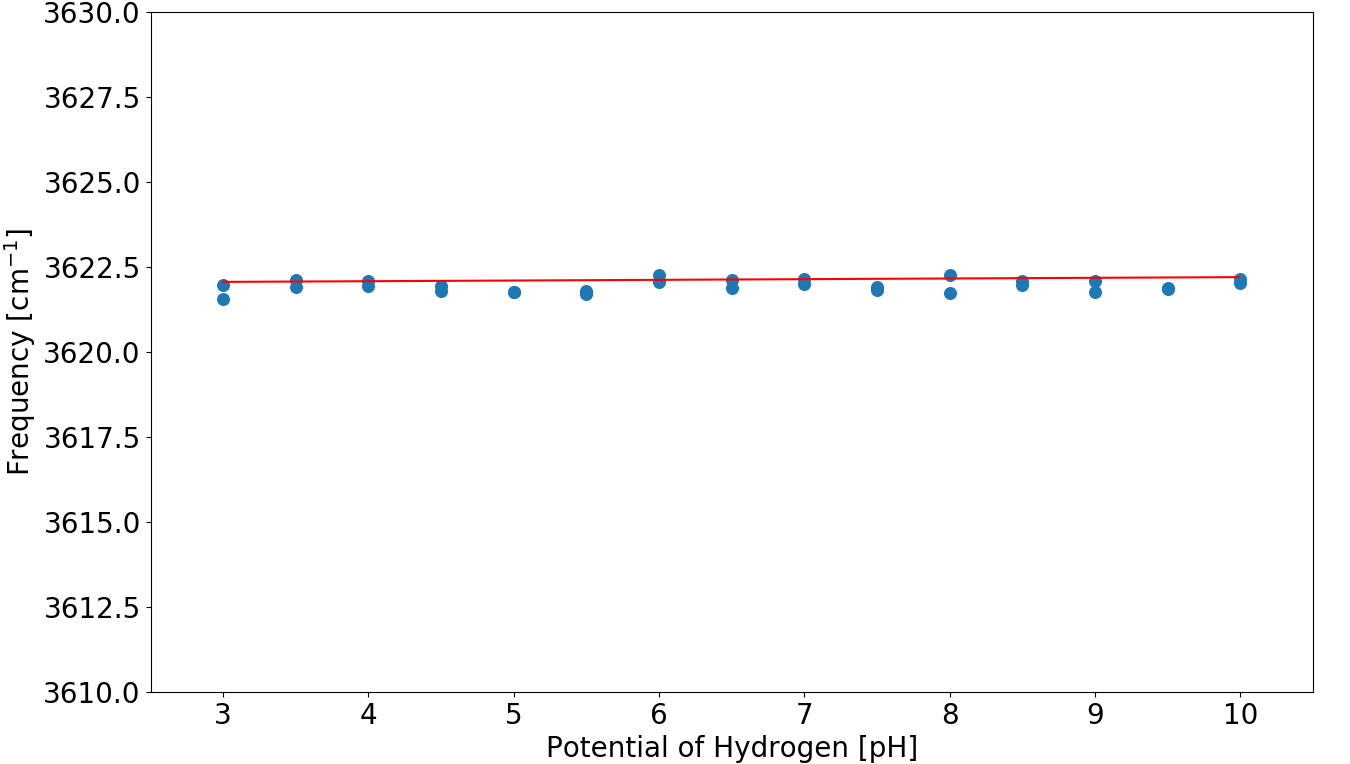
\includegraphics[scale=0.5]{images/hydrx_shift.png}
	\caption{Structural O-H stretching mode frequencies of the Li sample series from Belle Fourche bed F as a function of the pH. Each 0.5 pH interval has two data points. Linear regression provided only as a guide to the eye.}
	\label{fig:hydroxyl_shift}
\end{figure}

The observed shifts in the structural O-H mode had even fewer variations, remaining almost constant with changes in the pH. Figure~\ref{fig:hydroxyl_shift} demonstrates this for the Belle Fourche bed F, Li series. The line provided as a guide is notably more horizontal than for the previously mentioned $\nu_2$ mode. Same sample series were less constant however, having lower resonance frequencies at lower pH values. These differences were not usually more than 2$cm^{-1}$ from the max value which was quickly reached as the pH increased. The range of frequencies over which this mode was observed for each series may be found in Table~\ref{tab:structural_shifts}.

\begin{table}
	\centering
	\caption{The frequencies over which the shift in the structural O-H stretching mode occurs when moving from pH of 3 to 10 for all sample series.}
	\label{tab:structural_shifts}
	\begin{tabular}{|c||c|}
		\hline
		\textbf{Sample Series} & \textbf{Frequency Range of Structural O-H Mode [$\bm{cm^{-1}}$]} \\
		\hline
		\hline
		Li $_A$ & 3624 - 3625 \\
		\hline
		Li $_C$ & 3624 - 3627 \\
		\hline
		Li $_F$ & 3622 \\
		\hline
		Li $_T$ & 3621 - 3624 \\
		\hline
		Na $_A$ & 3624 - 3626 \\
		\hline
		Na $_C$ & 3626 - 3630 \\
		\hline
		Na $_F$ & 3622 \\
		\hline
		Na $_M$ & 3624 - 3626 \\
		\hline
		Na $_T$ & 3624 - 3625 \\
		\hline
		K $_A$ & 3624 - 3626 \\
		\hline
		K $_C$ & 3627 - 3630 \\
		\hline
		K $_M$ & 3624 - 3627 \\
		\hline
		K $_T$ & 3622 - 3626 \\
		\hline
	\end{tabular}
\end{table}

\begin{figure}
	\centering
	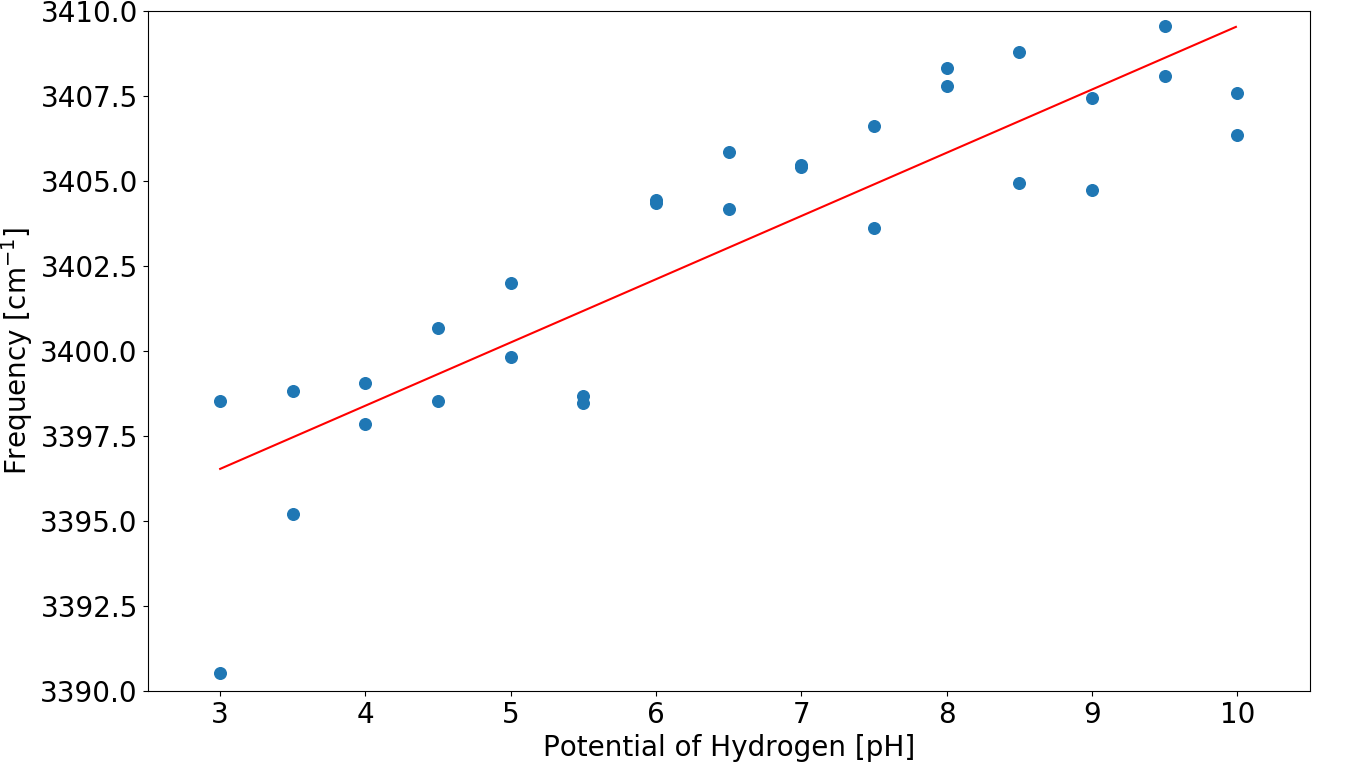
\includegraphics[scale=0.5]{images/water_shift.png}
	\caption{Symmetric O-H water stretching mode frequencies of the Li sample series from Belle Fourche bed F as a function of the pH. The linear regression is only provided as a guide to the eye.}
	\label{fig:water_shift}
\end{figure}
\begin{figure}
	\centering
	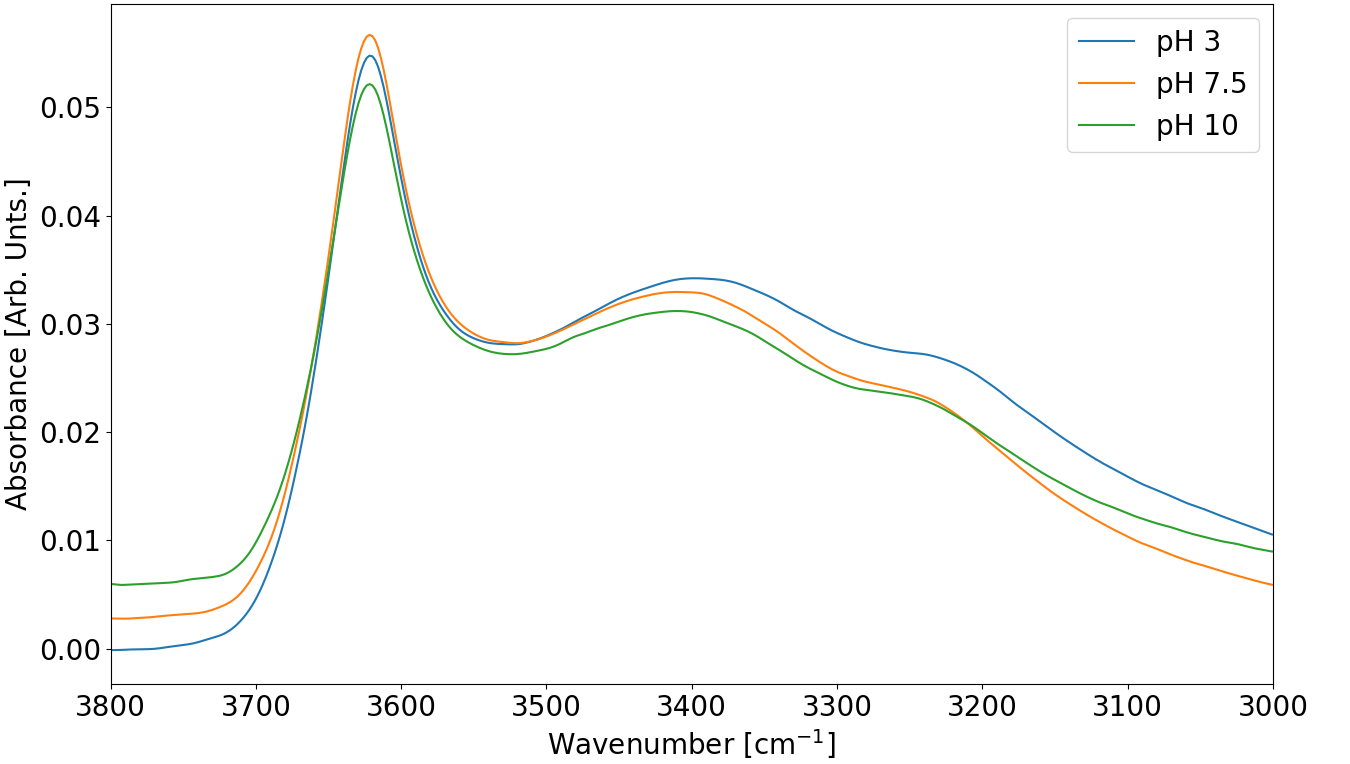
\includegraphics[scale=0.5]{images/spectra_shifts.png}
	\caption{Three spectra from the Belle Fourche F Li series, with visible shift in location of $\nu_1$ mode.}
	\label{fig:spectra_shift}
\end{figure}

We now arrive at the frequency shift of the $\nu_1$ mode as a function of pH, presented in Figure~\ref{fig:water_shift}. There are stark differences between this plot and the two immediately preceding it. The frequency of this mode clearly increases as the pH is increased from 3 to 10, by approximately 13$cm^{-1}$ in the presented case, much larger than the 2$cm^{-1}$ resolution. This general trend to increase in frequency was visible in all sample series for all exchangeable cations, and origin locations. Other Li sample series demonstrated much greater shifts though, sometimes 19$cm^{-1}$ or 25$cm^{-1}$ over the 3 - 10 pH range. A second visual outlining the shift in the $\nu_1$ mode is provided in Figure~\ref{fig:spectra_shift}. One can easily see how the smaller absorbance peaks attributed to the $\nu_1$ mode are not aligned, while the absorbance peaks for the structural O-H stretching mode are all perfectly aligned. Table~\ref{tab:stretch_shifts} provides the value for what was determined to be the average shift in frequency for the $\nu_1$ mode, determined by linear regression.

\begin{table}
	\centering
	\caption{Average frequency shifts for the three investigated modes of all Li sample series, found using linear regressions. The subscript represents which mine bed the series came from (Belle Fourche A,C,F, Treherne, and Miniota).}
	\label{tab:stretch_shifts}
		\begin{tabular}{|c||c|}
			\hline
			\textbf{Sample Series} & \textbf{Frequency Shift in $\bm{\nu_1}$ Mode [$\bm{cm^{-1}}$]} \\
			\hline
			\hline
			Li $_A$ & 13.99 \\
			\hline
			Li $_C$ & 25.76 \\
			\hline
			Li $_F$ & 13.04 \\
			\hline
			Li $_T$ & 19.18 \\
			\hline
			Na $_A$ & 22.73 \\
			\hline
			Na $_C$ & 20.33 \\
			\hline
			Na $_F$ & 17.77 \\
			\hline
			Na $_M$ & 40.08 \\
			\hline
			Na $_T$ & 30.27 \\
			\hline
			K $_A$ & 17.82 \\
			\hline
			K $_C$ & 7.72 \\
			\hline
			K $_M$ & 15.66 \\
			\hline
			K $_T$ & 33.43 \\
			\hline
	\end{tabular}
\end{table}

\subsection{Discussion}

From Table~\ref{tab:deformation_shifts}, one can see that all sample series had water deformation modes which occurred between 1628 and 1630 $cm^{-1}$. Typically, as with the Li series from Belle Fourche F bed,  the frequency of the $\nu_2$ mode had a slight shift, starting at the lower end of this 2$cm^{-1}$ band at pH 3, and moving to the 1630$cm^{-1}$ end at a pH of 10. Given the resolution was 2$cm^{-1}$, this slight shift can not be considered significant. That being said, most Li sample series displayed a similar trend as well, on the same order of magnitude. More experiments should be conducted to examine this region with a higher resolution, to see if this shift is of significance or not.

The frequency of the structural O-H hydroxyl group stretching had somewhat similar properties, in that the frequency remained quite constant over the range of pH values tested. At the lower range of tested pH values, this frequency was sometimes also lower than for the samples at higher pH values, by approximately 1 - 1.5 $cm^{-1}$. By pH values of 5 or higher, the frequency of this mode was constant, if it had appeared at lower frequencies for lower pHs. As the shifts were within the 2$cm^{-1}$ resolution of the measurements, and many series didn't have any measurable variation from the average value of the frequency, these slight shifts can not be considered significant. While the water deformation mode had the same frequencies for every sample series examined, the average frequency for the structural O-H stretching mode was not constant between sample series from different clay mines. At first glance one would think there is no trend. Upon further inspection however, it was realized that the frequency of this mode actually has a dependence on the clay mine, where the original clay powder for the samples was collected. Regardless of pH or exchangeable cation, series which came from the same clay mine tended to have very similar O-H stretching frequencies of their hydroxyl groups. Assuming clays which come from the same location have a similar structure in terms of substitutions and composition apart from the species of exchangeable cation, the exact frequency of this mode depends on the composition of the clay structure itself.

Shifts in the symmetric stretching mode of water, seen in Table~\ref{tab:stretch_shifts}, are blatantly different from the two previously examined modes however. While the deformation and the structural O-H stretching modes showed no significant variation with changes in the pH, the frequency of the $\nu_1$ mode did present with a variation which was visible in all sample series. Shifts ranging from 13$cm^{-1}$ up to 40$cm^{-1}$ were observed, often being ten times larger than the resolution. These shifts were obtained using a linear regression, though it should be noted that this method was used for its simplicity, and it not meant to describe any known theory. Regardless of cation species or clay mine, there was always a strong positive shift. It should be noted however that the correlation of the data was much better for the Li and Na sample series, than for the K series. This has been attributed to the K samples having less water, as previously discussed.


%%% Local Variables: 
%%% mode: latex
%%% TeX-master: t
%%% End: 
